\begin{enunciado}{2}
    Show that for the learning model of positive rectangles (aligned horizontally or vertically), $m_{\hipotset}(4) = 2^4$ and $m_{\hipotset}(5) < 2^5$. Hence, give a bound for $m_{\hipotset}(N)$.
\end{enunciado}

In order to show that the VC dimension is 4 (in this case), we need to show two things:

\textbf{1. There exist 4 points that can be shattered}
It’s clear that capturing just 1 point and all 4 points are both trivial. The figure below shows how we
can capture 2 points and 3 points.

\begin{figure}[h]
	\centering
	\begin{minipage}{0.46\textwidth}
		\centering
		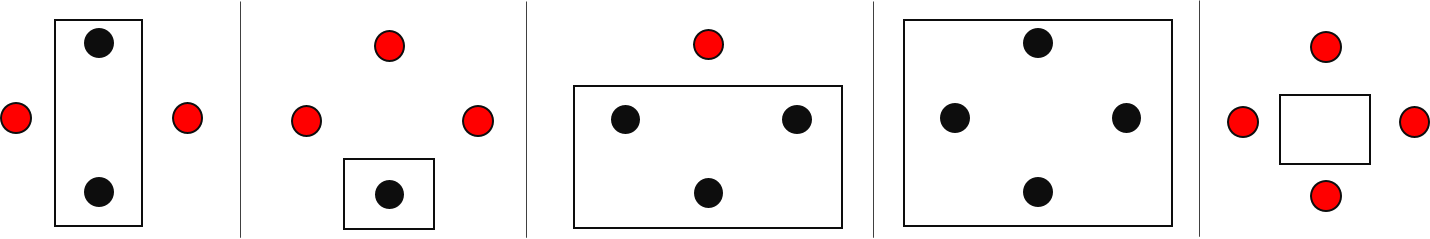
\includegraphics[width=\textwidth]{images/2-2-dvc4.png}
		\caption{arrangement of 4 points that can be shattered}
	\end{minipage}
\end{figure}

\textbf{2. No set of 5 points can be shattered}

Suppose we have 5 points. A shattering must allow us to select all 5 points and allow us to select 4
points without the 5th.

\begin{figure}[h]
	\centering
	\begin{minipage}{0.45\textwidth}
		\centering
		
\includegraphics[width=\textwidth]{images/2-2-dvc5.png}
		\caption{arrangement of 4 points that can be shattered}
	\end{minipage}
\end{figure}

Our minimum enclosing rectangle that allows us to select all five points is defined by only four points
– one for each edge. So, it is clear that the fifth point must lie either on an edge or on the inside of
the rectangle. This prevents us from selecting four points without the fifth.